\documentclass[acmsmall,screen,review]{acmart}
%%%%%%%%%%%%% Packages
\usepackage[utf8]{inputenc}
\usepackage{xcolor}
\usepackage{mathpartir}
\usepackage{tikz}
\usepackage{hyperref}
\usepackage{cleveref}
\usepackage{subcaption}
\graphicspath{{figures/}}
\usepackage{changepage}
\usepackage{etoolbox}
\usepackage{booktabs}
\usepackage{listings}
\usepackage{xspace}
\usepackage[true]{anonymous-acm} % For anonymous submission; change to 'false' for camera-ready
\usetikzlibrary{shapes.geometric, shapes.multipart, arrows.meta, positioning, calc, backgrounds, patterns, decorations.pathreplacing}

%%%%%%%%%%%%%% Comments
\usepackage[]{comments} % add option 'hide' to hide all
\Commenter{lef}

%%%%%%%%%%%%% Reference macros
\newcommand{\sect}[1]{Section~\ref{#1}\xspace}
\newcommand{\figr}[1]{Figure~\ref{#1}\xspace}
\newcommand{\tabl}[1]{Table~\ref{#1}\xspace}
\newcommand{\defn}[1]{Definition~\ref{#1}\xspace}
\newtheorem{definition}{Definition}

%%%%%%%%%%%%% Custom terms
\newcommand{\hadl}{HADL\xspace}


%% Listings setup for HADL code examples
\usepackage{listings}
\usepackage{color}
\lstdefinelanguage{hadl}{
  keywords={workflow, let, var, tool, agent, ask, say, if, else, while, for, in, type, enforce, eval, as, js},
  keywordstyle=\bfseries,
  sensitive=true,
  comment=[l]{//},
  morestring=[b]",
  stringstyle=\itshape,
}
\lstset{
  basicstyle=\ttfamily\small,
  columns=flexible,
  keepspaces=true,
  showstringspaces=false,
  numbers=left,
  numberstyle=\tiny\color{gray},
  numbersep=5pt,
  xleftmargin=2em,
  frame=single,
  framesep=3pt,
  aboveskip=1em,
  belowskip=1em,
  escapeinside={(*@}{@*)},
}

%% Bibliography style
\citestyle{acmauthoryear}

%% Remove ACM-specific metadata for submission
\settopmatter{printfolios=true,printccs=false,printacmref=true}

%% Document metadata
\acmJournal{PACMPL}
\acmVolume{0}
\acmNumber{PLDI}
\acmArticle{0}
\acmYear{2026}
\acmMonth{6}
\acmDOI{}

%% Copyright - for submission
\setcopyright{none}

\begin{document}

\title{Hierarchical Agentic Dataflow Language: Plans All the Way Down}

\authoranon{
\author{First Author}
\affiliation{%
  \institution{Institution}
  \city{City}
  \state{State}
  \country{Country}
}
\email{first@example.com}

\author{Second Author}
\affiliation{%
  \institution{Institution}
  \city{City}
  \state{State}
  \country{Country}
}
\email{second@example.com}
}

\keywords{domain-specific languages, agentic workflows, gradual typing, authorization, Cedar, LLM agents}

\begin{abstract}
  Agentic workflows built with existing orchestration frameworks lack static type checking, express control flow through graph construction rather than imperative constructs, and treat authorization as an external concern. We present HADL, a typed imperative domain-specific language in which human interaction, LLM tool invocation, and LLM reasoning are first-class typed expressions composable with mutable state, unbounded loops, structured iteration, and nested workflow composition. The central mechanism is \emph{gradual generation}, in which LLMs produce not only values but also types, workflows, and authorization policies at runtime. The \texttt{Schema} type is universally compatible during static checking and triggers staged re-typechecking when concrete types materialize at runtime. Arrow types enable LLM-generated workflows to be deserialized and executed via \texttt{eval} with type checking at the call site. The \texttt{Policy} type enables LLM-generated Cedar policies to be activated via an explicit \texttt{enforce} expression, with safety checks that reject deny-all rules and invalid action types, scoped principal validation, and append-only merging that can only tighten access. All three forms share provenance-driven self-healing that re-invokes the causal tool call when validation fails. The language is implemented in Rust with PEG parsing, static type checking, and async tree-walking interpretation.
\end{abstract}

\maketitle

\section{Introduction}
\label{sec:intro}

Modern agents write substantial programs. A single agent run now sequences many gen calls, branches on intermediate results, accumulates mutable state, and delegates subtasks to other agents. The volume of code an agent authors grows with every model generation. What does not grow is safety. A workflow of ten gen calls receives no more type discipline than a one-shot prompt, and authorization, when enforced at all, is applied at the outer boundary rather than at each call. The gap shows up on the two axes that matter. Gen outputs flow from one call to the next with no check that their shape matches what downstream code expects, and sensitive gens can be invoked from within a workflow with no evidence that the invocation was authorized. As agents are trusted with more consequential work such as filling forms, querying sensitive records, and generating other agents, safety must scale with the size of the workflow rather than lag behind it.

Our position is simple. Agents plan, and plans are programs. If plans are programs, then the mature body of programming-language techniques applies directly to them. Type systems discipline the data flowing between gen calls. Gradual typing~\cite{siek2006gradual} accommodates the values, types, workflows, and policies that only materialize at runtime when the LLM produces them. Static analysis catches structural errors before any LLM call is paid for, and authorization semantics let each gen invocation be checked against an explicit principal. The same type and gen-call information that constrains what the LLM may produce also shapes how it generates, so the infrastructure that catches errors is the infrastructure that prevents them. Safety that scales with the size of the workflow is exactly what these techniques deliver. Every new gen call, every new field access, and every new principal is another point at which the program can be checked.

Today developers express these plans using orchestration frameworks such as LangChain~\cite{langchain2022} or ad-hoc Python scripts. These approaches treat plans as configurations of library objects rather than as programs in their own right. Gen calls return untyped data, control flow is scattered across callback edges, structural errors surface only at runtime, and authorization is applied at the outer boundary rather than per invocation. Neighboring programming-language approaches such as LMQL~\cite{beurer2023prompting} and DSPy~\cite{khattab2023dspy} address parts of this problem but do not integrate a type system for gen outputs with per-invocation authorization. Yue et al.~\cite{yue2026statictemplatesdynamicruntime} identify the tension between expressivity and verifiability as a central open problem in this space.

\begin{figure}[H]
\begin{lstlisting}[language=hadl,showstringspaces=false]
@retries 3

workflow clinical_trial() -> String {
  let trial  = ask "Describe the clinical trial"
  let crf: Schema   = gen "Generate a CRF schema for `trial`"
  let policy: Policy = gen "Coordinators cannot see data in
    unblinded folder. Safety board has full access."
  enforce policy
  let num_visits = ask "How many patient visits to simulate?"
  let pids: Schema = gen "Return `num_visits` patient IDs"
  var cost: Number = 0
  for pid in pids {
    let visit: crf = gen "Generate a visit for `pid` in `trial`
      conforming to schema `crf`" as "coordinator"
    cost = js cost + visit.cost
    say "Visit `visit.patient_id`: cost `visit.cost`"
  }
  agent "Write a report for the trial visits" as "safety_board"
}
\end{lstlisting}
\caption{Clinical-trial workflow demonstrating gradual schema typing (\texttt{crf} typed binding),
  gradual policy typing (\texttt{enforce policy}), and per-invocation Cedar authorization (\texttt{as} clause).
  \texttt{@retries 3} activates feedback-driven self-healing: if the generated schema lacks a field
  accessed later (\texttt{visit.cost}, \texttt{visit.patient\_id}), the runtime retries the causal
  \texttt{gen} with the violated constraint as feedback before any visit data is collected.}
\label{fig:clinical-trial}
\end{figure}


Figure~\ref{fig:clinical-trial} illustrates gradual validation and per-invocation authorization in a single workflow. Two \texttt{gen} calls produce program structure, a type used in later bindings and a policy activated via \texttt{enforce} on the next line. Every subsequent \texttt{gen} and \texttt{agent} call is typed against the generated schema and checked against the generated policy under an explicit principal, including the closing \texttt{agent} call that returns an LLM-written summary. The same type discipline that governs ordinary field access such as \texttt{visit.patient\_id} governs the LLM output that produced the value.

We present HADL (Hierarchical Agent Dataflow Language), a strongly typed imperative domain-specific language for composing long-running agentic workflows. HADL provides four domain-specific primitives, \texttt{ask}, \texttt{say}, \texttt{gen}, and \texttt{agent}, as first-class typed expressions in an imperative language with mutable state, unbounded loops, structured iteration, and nested workflow composition. The type system supports three forms of gradual validation. The \texttt{Schema} type lets a gen produce a type that resolves to a concrete type once the LLM delivers one, after which subsequent uses are checked under the same type system. Workflow types let a gen produce a complete workflow that is then invoked via \texttt{eval} and checked at the call site. The \texttt{Policy} type lets a gen produce a Cedar~\cite{cutler2024cedar} policy that is then activated via \texttt{enforce}, with safety checks and append-only merging so that activation can only tighten access. The language and runtime are implemented in Rust, integrating with the GitHub Copilot SDK for LLM execution.

This paper makes two contributions.

\begin{enumerate}
	\item We design HADL, an imperative DSL in which \texttt{ask}, \texttt{say}, \texttt{gen}, and \texttt{agent} are first-class typed expressions with curried function types, providing natural imperative syntax for multi-turn agent orchestration. A type checker with source-span diagnostics catches structural errors before any LLM call is made. The language is implemented in Rust with a PEG parser, type checker, and async tree-walking interpreter.
	\item We introduce \emph{gradual validation}, a mechanism in which types, workflows, and policies are produced by LLMs and checked at runtime. Beyond catching errors, the declared types guide the LLM's generation itself, so every call produces output shaped to fit the surrounding program. \texttt{Schema} resolves to a concrete type once an LLM produces one, after which subsequent uses are checked under the same type system. Workflow types enable LLM-generated workflows executed via \texttt{eval}. \texttt{Policy} enables LLM-generated Cedar authorization policies activated via \texttt{enforce}, with a deny-all guard, scoped principal validation, and append-only merging. All three share provenance-driven self-healing that reruns the generator when validation fails.
\end{enumerate}

The remainder of this paper is organized as follows. Section~\ref{sec:overview} presents the language through motivating examples. Section~\ref{sec:design} presents the type system and gradual validation. Section~\ref{sec:semantics} gives the operational semantics and states soundness. Section~\ref{sec:implementation} describes the compilation pipeline and runtime. Section~\ref{sec:related} discusses related work, and Section~\ref{sec:conclusion} concludes.

\section{Overview}
\label{sec:overview}

We introduce HADL through two self-contained workflows. The first covers types and policies, showing how values, types, and authorization rules produced by the LLM are validated under the same type discipline and authorization semantics that govern the rest of the program. The second covers workflow generation, showing how a \texttt{gen} call can produce a complete HADL workflow that executes as part of the workflow that produced it. Together, the two workflows cover HADL's main contributions before the formal treatment in Sections~\ref{sec:design} and~\ref{sec:implementation}.

HADL programs consist of workflow declarations, which are typed functions that compose four domain-specific primitives with standard imperative constructs. The primitive \texttt{ask} prompts a human operator and returns a \texttt{String}. The primitive \texttt{say} prints a string to the output stream and returns unit. The primitive \texttt{gen} sends a description to an LLM gen session configured to return structured data and requires an explicit type annotation at the binding site. The primitive \texttt{agent} sends an instruction to an LLM reasoning session and returns a \texttt{String}. These four primitives are first-class expressions in the language, not callbacks or graph nodes, so they compose naturally with \texttt{let} and \texttt{var} bindings, \texttt{if}/\texttt{else} branches, \texttt{while} loops, \texttt{for} iteration, and inline JavaScript expressions via the \texttt{js} keyword. The type checker runs before execution begins, rejecting \texttt{gen} calls without type annotations, assignments to immutable variables, and return type mismatches, all with diagnostic source spans.

\subsection{Gradual Validation for Types and Policies}
\label{sec:overview-types-policies}

Many agentic workflows need to handle two kinds of runtime information at once. The shape of the data flowing between \texttt{gen} calls is not known until the LLM produces it, and the authorization rules that govern those calls are often specific to the operator, the task, or the stage of the workflow. HADL handles both with the same type discipline. The \texttt{Schema} type is compatible with every static type and resolves to a concrete type once the LLM delivers one, after which the rest of the program is checked under the same type system. The \texttt{Policy} type binds an LLM-generated Cedar policy as a value, and an explicit \texttt{enforce} expression activates it, after which every subsequent \texttt{gen} or \texttt{agent} invocation is checked against a principal supplied at the call site.

Figure~\ref{fig:clinical-trial} shows a clinical trial workflow. The \texttt{@retries 3} pragma on line~1 activates self-healing, described below. Line~4 prompts the operator for a trial description. Line~5 binds \texttt{crf} with a \texttt{Schema} annotation, signalling to the type checker that this variable will hold a type produced at runtime. When line~5 executes, the interpreter parses the LLM's response as a JSON Schema value, converts it to a concrete HADL type, and checks the remainder of the program against that concrete type under the same type discipline that governs the rest of the language. Line~6 produces a blinding policy and line~8 activates it with \texttt{enforce}. After line~8, every \texttt{gen} and \texttt{agent} invocation constructs an authorization triplet with its declared principal and is checked against the installed policy before any LLM call is made. Line~10 asks the LLM for a list of patient identifiers, bound as \texttt{Schema} since the array structure is determined at runtime. The \texttt{for} loop on lines~12--16 iterates that list. Line~13 binds \texttt{visit} with type \texttt{crf}, so the output is validated against the concrete schema produced on line~5, and the field access \texttt{visit.patient\_id} on line~15 is checked under the same type system. The \texttt{gen} call inside the loop carries the \texttt{as role} clause, so each invocation is authorized for the principal the operator declared on line~9, and line~14 counts each successful visit in the mutable \texttt{total} via an inline \texttt{js} expression. If a serious adverse event is reported, lines~20--21 produce and activate a second policy. The two policies are merged append-only, so access rules only tighten. Line~22 can only run when the principal is \texttt{safety\_board}, because the merged policy blocks every other role from adverse event reports.

The \texttt{@retries} pragma activates self-healing. When validation rejects an LLM output, the runtime identifies the \texttt{gen} call that produced the rejected value, re-invokes it with the violated constraint appended to the original prompt, and re-runs the check under the same type and authorization discipline. The loop runs up to the declared retry limit. If the retry limit is exhausted, the interpreter raises the underlying error with the full diagnostic.

\subsection{Gradual Validation for Workflow Generation}
\label{sec:overview-workflow}

Agentic workflows often delegate subtasks whose structure is itself the subject of the current reasoning step. A scoring function, a triage procedure, or a data cleaning pipeline may all be worth producing on the fly, shaped by what the operator has just said. HADL handles this by making workflows first-class values with arrow types. When a \texttt{gen} call is annotated with an arrow type, the LLM produces a complete HADL workflow as a JSON-serialized AST, and the \texttt{eval} expression deserializes and invokes it in the calling workflow's environment. The generated workflow is not a separate program. It runs as part of the workflow that produced it, sharing the caller's variable scope, and every \texttt{eval} site is checked against the arrow's parameter and return types.

Figure~\ref{fig:overview-workflow} shows a car recommendation workflow and the workflow it produces. Line~3 of the outer workflow generates a \texttt{Schema} describing a single car. Line~4 asks the LLM to generate a scorer with the arrow type \texttt{(car\_schema -> Number)}, an arrow whose parameter type is the runtime-generated \texttt{car\_schema} itself. The LLM produces the workflow shown below the arrow, taking a car conforming to the schema and returning a numeric score. The \texttt{while} loop on lines~9--18 fills the schema three times, binding a fresh \texttt{car} value with type \texttt{car\_schema} on each iteration so that every LLM output is validated against the concrete shape produced on line~3. Line~11 applies the generated scorer via \texttt{eval scorer(car)}. At the \texttt{eval} expression the type checker verifies that the argument type matches the arrow's parameter type and that the result is used where the return type is accepted. Line~14 extracts the car's name via an inline \texttt{js} expression when a new best score is found. The arrow between the two listings indicates that the generated workflow is produced by the \texttt{gen} call on line~4 of the outer workflow and runs in the same interpreter context. The generated workflow itself calls \texttt{gen} three times to rate comfort, cost, and reliability, and uses an inline \texttt{js} expression to average the three ratings.

\begin{figure}[H]
\centering
\begin{subfigure}{\linewidth}
\begin{lstlisting}[language=hadl,showstringspaces=false]
workflow pick_car() -> String {
  let prefs = ask "What matters most?"
  let car_schema: Schema = gen "Schema for a car with name and type"
  let scorer: (car_schema -> Number) = gen "Workflow that
    scores a car on `prefs`"
  var best: String = ""
  var top: Number = 0
  var i: Number = 0
  while (i < 3) {
    let car: car_schema = gen "Fill the schema with a popular car"
    let score: Number = eval scorer(car)
    if (score > top) {
      top = score
      best = js car.name
    }
    say "`car.name` rated `score`"
    i = js i + 1
  }
  say "Recommended `best`"
  best
}
\end{lstlisting}
\subcaption{Outer workflow.}
\end{subfigure}

\vspace{0.4em}
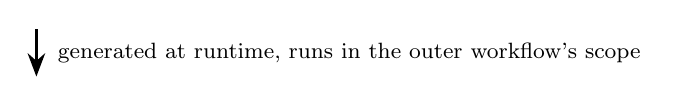
\begin{tikzpicture}[>=Stealth]
  \draw[->, very thick] (0,0.3) -- (0,-0.3);
  \node[right, font=\footnotesize] at (0.15,0)
    {generated at runtime, runs in the outer workflow's scope};
\end{tikzpicture}
\vspace{0.4em}

\begin{subfigure}{\linewidth}
\begin{lstlisting}[language=hadl,showstringspaces=false]
// produced by the gen call on line 4 above
workflow score(car: car_schema) -> Number {
  let comfort: Number = gen "Rate comfort of `car.name`"
  let cost: Number = gen "Rate cost of `car.name`"
  let reliability: Number = gen "Rate reliability of `car.name`"
  js (comfort + cost + reliability) / 3
}
\end{lstlisting}
\subcaption{Generated workflow.}
\end{subfigure}
\caption{A car recommendation workflow illustrating gradual validation for workflow generation. Line~3 of the outer workflow generates a schema for a single car. Line~4 asks the LLM for a scorer with arrow type \texttt{(car\_schema -> Number)}, the parameter being the runtime-generated type itself. The LLM produces the workflow shown below, taking a car that conforms to the schema and returning a numeric score. The \texttt{while} loop fills the schema three times, and \texttt{eval scorer(car)} on line~11 invokes the generated workflow for each fresh car, evaluating it in the outer workflow's variable scope. At every \texttt{eval} site, the type checker verifies that the argument matches the arrow's parameter type and that the result is used where the return type is accepted. The generated workflow itself calls \texttt{gen} three times and averages the results with an inline \texttt{js} expression, showing that a generated workflow has full access to HADL's primitives and JavaScript interop.}
\label{fig:overview-workflow}
\end{figure}

\section{Design}
\label{sec:design}

This section presents the \pact type system and the gradual validation mechanism
that unifies type generation, workflow generation, and policy generation. We
describe the abstract syntax, the correspondence between \pact types and
JavaScript types, and the three forms of gradual validation that check
LLM-produced types, programs, and authorization policies at runtime.
\sect{sec:semantics} gives the operational semantics and soundness theorem.

\subsection{Syntax}
\label{sec:design-syntax}

\begin{sloppypar}
Figure~\ref{fig:syntax} presents the abstract syntax. A program is pragmas
followed by declarations. Types include base types (now including
\texttt{Principal} and \texttt{Path}), \texttt{Schema}, arrow types,
\texttt{Policy}, and named references. Expressions add to standard imperative
constructs the four primitives, \texttt{eval}, \texttt{enforce}, comparisons,
and the principal introducers \texttt{root} and \texttt{restrict}\;$e$. The
\texttt{as} clause on \texttt{gen}/\allowbreak\texttt{agent} takes an expression
of type \texttt{Principal}; the legacy literal-string form is dropped in favor
of named principals (\texttt{let user: Principal = restrict root}).
\end{sloppypar}

\begin{figure}[t]
\[\begin{array}{rcll}
P & ::= & \pi^*\; d^* & \textit{program} \\[4pt]
\pi & ::= & \texttt{@policy}\; s & \textit{policy pragma} \\
    & \mid & \texttt{@retries}\; n & \textit{retry pragma} \\[4pt]
d & ::= & \texttt{workflow}\; f(\overline{x_i{:}T_i}) \to T\; \{e\} & \textit{workflow declaration} \\
  & \mid & \texttt{type}\; X = T & \textit{type declaration} \\[4pt]
T & ::= & () \mid \texttt{String} \mid \texttt{Number} \mid \texttt{Bool} & \textit{base types} \\
  & \mid & \texttt{Schema} & \textit{type of types} \\
  & \mid & \texttt{Policy} & \textit{authorization policy} \\
  & \mid & (T_1 \to T_2) & \textit{arrow type} \\
  & \mid & \texttt{array[}T\texttt{]} & \textit{array type} \\
  & \mid & \{ \overline{x_i{:}T_i} \} & \textit{record type} \\
  & \mid & X & \textit{named type reference} \\[4pt]
e & ::= & s \mid n \mid b & \textit{literals} \\
  & \mid & x & \textit{variable reference} \\
  & \mid & \texttt{let}\; x {:} T = e \mid \texttt{let}\; x = e & \textit{immutable binding} \\
  & \mid & \texttt{var}\; x {:} T = e \mid \texttt{var}\; x = e & \textit{mutable binding} \\
  & \mid & x = e & \textit{assignment} \\
  & \mid & \texttt{if}\; (e)\; \{e\}\; [\texttt{else}\; \{e\}] & \textit{conditional} \\
  & \mid & \texttt{while}\; (e)\; \{e\} & \textit{loop} \\
  & \mid & \texttt{for}\; x\; \texttt{in}\; e\; \{e\} & \textit{iteration} \\
  & \mid & \texttt{ask}\; s & \textit{human prompt} \\
  & \mid & \texttt{say}\; s & \textit{human output} \\
  & \mid & \texttt{gen}\; s\; [\texttt{as}\; (s \mid x)] & \textit{LLM gen call} \\
  & \mid & \texttt{agent}\; s\; [\texttt{as}\; (s \mid x)] & \textit{LLM agent call} \\
  & \mid & \texttt{js}\; c & \textit{JavaScript expression} \\
  & \mid & \texttt{eval}\; e\;(e_1, \ldots, e_k) & \textit{workflow invocation} \\
  & \mid & \texttt{enforce}\; x & \textit{policy activation} \\
  & \mid & e_1 \;\mathit{op}\; e_2 & \textit{comparison} \\
  & \mid & e_1 ;\; e_2 & \textit{sequencing} \\[4pt]
\mathit{op} & ::= & \texttt{==} \mid \texttt{!=} \mid \texttt{<} \mid \texttt{<=} \mid \texttt{>} \mid \texttt{>=} & \textit{comparison operators}
\end{array}\]
\caption{Abstract syntax of Pact. Optional components are in square brackets and $\overline{x_i{:}T_i}$ denotes a possibly empty sequence.}
\label{fig:syntax}
\end{figure}

\begin{sloppypar}
\pact's base types correspond to JavaScript types
($\texttt{String}{\to}\texttt{string}$, etc.), and all runtime values are
represented as JSON. The type checker uses inference with subsumption.
\texttt{gen} is oracular, requiring explicit annotations at binding sites. Three
types play a special role in gradual validation: \texttt{Schema} is the
\emph{type of types}, arrow types are the types of workflows, and
\texttt{Policy} is the type of authorization rules. All three share the property
that their concrete values are generated by the LLM at runtime.
\end{sloppypar}

\subsection{Gradual Validation}
\label{sec:design-gradual}

The three gradual-validation annotations, namely \texttt{Schema},
arrow types, and \texttt{Policy}, share the same mechanism. Static
checking defers structural constraints on these types until the LLM
produces a concrete value at runtime, inspired by gradual
typing~\cite{siek2006gradual}. Rather than inserting
casts, \pact{} re-invokes the type checker over downstream code when a
concrete value materializes.

The common pattern is that an LLM-produced artifact is first accepted
only at an abstract type and is later forced when the program reaches a
use site that depends on its concrete structure. At that point, \pact{}
does not merely check the artifact in isolation. It re-checks the
program region that depends on the artifact. If the check fails, the
runtime records the violated constraint and retries the generator that
produced the artifact. This makes the retry causal. A missing field in a
generated schema retries the schema generator, not each later value
generator that happens to expose the missing field. An ill-typed
generated workflow retries the workflow generator, not the caller. A
malformed generated policy retries the policy generator before the
policy is installed. Our base assumption is that the LLM is \emph{eventually
truthful} in the sense that it will produce a correct artifact within a bounded
number of retries (\defn{def:oracle-truthful}).

\paragraph{Gradual type generation.} A \texttt{gen} call producing a
\texttt{Schema} type produces a JSON Schema at runtime~\cite{jsonschema2020}. 
When a schema materializes, the
interpreter converts it to the corresponding \pact{} type, registers it, and
re-invokes the type checker over the remainder of the program. On failure
(within \texttt{@retries}) the runtime feeds the type error back to the causal
\texttt{gen}. See Appendix~\ref{app:gradual-detail} for the formalization
of the forward syntactic analysis and validation procedures.

\paragraph{Gradual workflow generation.} A \texttt{gen} call producing an arrow
type instructs the LLM to produce a complete \pact{} workflow as structured
output. Syntactic discrepancies are build-in and we can assume a \pact workflow will
be well-formed, but not necessarily well-typed. Workflow gradual validation then
takes effect, substituting the generated workflow at the call site (\texttt{eval}) and re-checking the caller's
continuation. On failure, the runtime retries the workflow generator with the error as feedback,
same as with gradual type generation. This is a powerful mechanism for
enforcing compositionality and modularity of LLM-generated workflows, which are otherwise black boxes. 
For example, in Figure~\ref{fig:overview-workflow} the workflow generator produces a subroutine that is called three times. 
If the generated workflow is ill-typed, the repair happens once at the source,
and all three calls conform on their first attempt. 

\paragraph{Gradual policy generation.} A \texttt{gen} call producing a
\texttt{Policy} type instructs the LLM to produce a Cedar policy as JSON. \pact
allows first class \emph{principals}---defined from others using the \texttt{restrict} command---
and \emph{policies}, generated by \texttt{gen} and activated by an \texttt{enforce} command later.
Separating generation from
activation lets a program generate a candidate policy, inspect it,
branch on it, or route it through human approval before it affects later
calls. A failed policy compile or authorization check triggers
feedback-driven self-healing.
Policy gradual validation checks that the generated policy is well-formed and
references only declared principals after it is enforced.
A failed validation retries the policy generator with
the error as feedback, before the policy is installed.

\paragraph{Cedar policies in \pact{}.} Cedar requests in \pact{} are
\texttt{(principal, action, resource)} triples with $\texttt{Action}\in
\{\texttt{Read},\texttt{Write},\texttt{Exec}\}$ and \texttt{Resource}
ranging over files and directories the agent ultimately touches;
wildcards \texttt{*} are supported in either slot. Principals form a
tree rooted at the top-level principal \texttt{root}; the policy
state begins as $\MPol_0 = \texttt{allow(root,\;*,\;*)}$ root is allowed
indiscriminate access to all files in the system, much like in the POSIX
model. Forbid policies are also allowed, for example \texttt{forbid(user, "Write", "/")}
prohibits the principal \texttt{user} from writing to any file. The policy state
is updated by appending new rules with the \texttt{enforce} command, and the
decision procedure is monotone in the deny direction.
The only way to create new principals is via \texttt{restrict}, which
creates a fresh child of an existing principal. 
$\texttt{let}\;b = \texttt{restrict}\;a$ declares $b$ as a fresh
descendant of $a$, inheriting all of $a$'s allowances by Cedar's
hierarchy semantics, for example one can create
a first principal by doing $\texttt{let}\;coordinator = \texttt{restrict}\;\texttt{root}$,
as seen in Figure~\ref{fig:clinical-trial}. Then a new policy
\texttt{enforce} admits only candidate policies in
which (i) every rule is forbid-effect, (ii) only principals
declared at the time the policy is enforced are referenced, and (iii) no rule references \texttt{root}.
These rules are required to prove the \emph{policy monotonicity} property of the runtime semantics, which states that the allow-set can only shrink across steps 
(Theorem~\ref{thm:pact-soundness}).
Because no rule can reference \texttt{root} and no rule can be allow-effect, no
rule can expand the authority of any principal, and because new principals are
created as descendants of existing ones,
no rule targets
\texttt{root}; together these admit only further restriction of
descendants from their inherited authority while leaving \texttt{root}
permanently maximal.

The static premise enforced at every \texttt{gen}/\texttt{agent} redex
is exactly $\PrinDeclared{\MPol}{\MPrin}$: the principal named in the
\texttt{as} clause, or \texttt{root} when none is given, is declared in
the current policy state. The action and resource of any specific
filesystem access become known only when the agent runs, so they are
checked just-in-time by the runtime monitor of
\sect{sec:implementation}.

\subsection{Threat Model and Limitations}
\label{sec:design-threat}

\pact{} trusts the programmer-authored text, the type checker, the
runtime re-checker, and the Cedar decision procedure, and treats every
LLM output as untrusted. The retry budget $\MRetry$ bounds how many
untrusted attempts the runtime consumes per site. Validation rejects
outputs that fail structural checks of the annotated type. Every
\texttt{gen}/\texttt{agent} carries the static premise
$\PrinDeclared{\MPol}{\MPrin}$ before the LLM is called, and every
filesystem access the agent then performs is policy-checked
just-in-time by the runtime monitor (\sect{sec:implementation}).
A type-validation failure triggers retry; a policy denial fails closed.

\paragraph{Authority is monotone in the deny direction.} Because
\texttt{enforce} installs only forbid-effect rules on non-root
principals (\sect{sec:design-gradual}), the allow-set
$\{(\MPrin, a, r) \mid \mathsf{allows}(\MPol, \MPrin, a, r)\}$
monotonically shrinks across every step. Generated policies can
therefore only restrict authority of declared descendants, never
expand it; this rules out privilege escalation through LLM-authored
policies as a class.

\label{sec:design-limitations}
Four threat classes remain outside this model.
These are prompt injection, semantic misalignment of generated policies,
\texttt{say}-based exfiltration, and host-side JavaScript effects.
They are expanded in \sect{app:threat}. Formal results are stated
relative to an \emph{eventually-truthful} oracle
(\defn{def:oracle-truthful}). An adversarial or permanently lying oracle
exhausts the budget and the configuration fails closed.
\sect{app:limitations} enumerates each restriction.

\section{Implementation}
\label{sec:implementation}

% TODO: Write implementation section

% \section{Evaluation}
\label{sec:evaluation}

We designed the following evaluation to answer four research questions raised by our claims about gradual validation. Numerical results are forthcoming; this section documents the experimental protocol, workflow corpus, metrics, and baseline-comparison methodology.

\subsection{Research Questions}
\label{sec:eval-rqs}

\begin{description}
  \item[RQ1 (validation rate).] How often do LLM-generated schemas, workflows, and policies pass \hadl's validator on first attempt, broken down by the three annotation types (\texttt{Schema}, arrow types, \texttt{Policy})?
  \item[RQ2 (self-healing convergence).] When first-attempt validation fails, does the bounded feedback-driven retry of \sect{sec:design-gradual} converge within the declared budget $\MRetry$, and at what retry depth?
  \item[RQ3 (overhead).] What is the latency and token-cost overhead of gradual validation and per-invocation Cedar authorization relative to an untyped orchestration baseline on the same workflow?
  \item[RQ4 (baselines).] For a representative typed-workflow task, how does \hadl compare quantitatively and qualitatively to LangGraph~\cite{langchain2022}, LMQL~\cite{beurer2023prompting}, and DSPy~\cite{khattab2023dspy}?
\end{description}

\subsection{Workflow Corpus}
\label{sec:eval-corpus}

The corpus contains six \hadl workflows, the two illustrative ones from \sect{sec:intro}--\sect{sec:overview} plus four new tasks chosen to exercise the three gradual-validation modes and per-invocation authorization under representative domain conditions.

\begin{table}[t]
\centering
\small
\begin{tabular}{@{}lrrrrl@{}}
\toprule
Workflow & LoC & \#\texttt{gen} & \#\texttt{Policy} & \#principals & Primary validation \\
\midrule
Clinical trial (\figr{fig:clinical-trial})       & 22 & 4 & 2 & 3 & \texttt{Schema}, \texttt{Policy} \\
Car scorer (\figr{fig:overview-workflow})        & \TODO{N} & \TODO{N} & \TODO{N} & \TODO{N} & arrow type \\
Customer-support triage                          & \TODO{N} & \TODO{N} & \TODO{N} & \TODO{N} & \texttt{Schema}, \texttt{Policy} \\
Code-review agent                                & \TODO{N} & \TODO{N} & \TODO{N} & \TODO{N} & arrow type, \texttt{Policy} \\
Financial-compliance report                      & \TODO{N} & \TODO{N} & \TODO{N} & \TODO{N} & \texttt{Schema}, \texttt{Policy} \\
Research-paper summarizer                        & \TODO{N} & \TODO{N} & \TODO{N} & \TODO{N} & \texttt{Schema} \\
\bottomrule
\end{tabular}
\caption{Workflow corpus. \emph{LoC} counts HADL source lines excluding comments. \emph{\#gen} is the static count of \texttt{gen} and \texttt{agent} call sites. \emph{\#Policy} is the number of \texttt{Policy}-typed bindings. \emph{\#principals} is the number of distinct roles named in \texttt{as} clauses.}
\label{tab:corpus}
\end{table}

\subsection{Methodology}
\label{sec:eval-method}

\paragraph{Models.} Each workflow is run against three LLMs: GPT-4.1, Claude-Sonnet-4, and the default model exposed by the GitHub Copilot SDK at the time of evaluation. All three are accessed through the same \hadl oracle interface.

\paragraph{Runs.} Each (workflow, model) pair is executed \TODO{$K$} times with distinct seeds and distinct synthetic user inputs drawn from a per-workflow input template, for a total of $6 \times 3 \times K$ runs. Workflows that depend on human input (\texttt{ask}) are driven by a scripted stub.

\paragraph{Retry budget.} All experiments fix $\MRetry = 3$, matching the \texttt{@retries 3} pragma on Figure~\ref{fig:clinical-trial} and within the practical range that our own deployments use.

\paragraph{Error taxonomy.} Every terminating run is classified as one of:
\begin{itemize}
  \item \emph{success} --- reduction reaches a value configuration;
  \item \emph{type rejection} --- an $\rulename{Oracle-Heal-Type}$ step consumed the full retry budget at some \texttt{gen} site;
  \item \emph{policy rejection} --- an $\rulename{Oracle-Heal-Pol}$ step consumed the full retry budget;
  \item \emph{policy-install failure} --- the deny-all guard or action-type check rejected an \texttt{enforce} policy after $\MRetry$ retries;
  \item \emph{runtime error} --- a non-oracle runtime exception (JS engine failure, network error).
\end{itemize}

\paragraph{Determinism controls.} For each (workflow, model) pair we record the full prompt sequence and the full oracle response trace. This lets us replay a failure deterministically for the post-mortem and makes the token-cost numbers of \sect{sec:eval-perf} reproducible.

\subsection{Results: Validation Rates (RQ1)}
\label{sec:eval-rates}

\begin{table}[t]
\centering
\small
\begin{tabular}{@{}lrrrrr@{}}
\toprule
Workflow & schema-pass & workflow-pass & policy-pass & retry-to-success & retry-exhausted \\
\midrule
Clinical trial            & \TODO{\%} & --- & \TODO{\%} & \TODO{\%} & \TODO{\%} \\
Car scorer                & --- & \TODO{\%} & --- & \TODO{\%} & \TODO{\%} \\
Customer-support triage   & \TODO{\%} & --- & \TODO{\%} & \TODO{\%} & \TODO{\%} \\
Code-review agent         & --- & \TODO{\%} & \TODO{\%} & \TODO{\%} & \TODO{\%} \\
Financial-compliance      & \TODO{\%} & --- & \TODO{\%} & \TODO{\%} & \TODO{\%} \\
Research-paper summarizer & \TODO{\%} & --- & --- & \TODO{\%} & \TODO{\%} \\
\bottomrule
\end{tabular}
\caption{Per-workflow first-attempt validation rates (\emph{schema-pass}, \emph{workflow-pass}, \emph{policy-pass} over all invocations of the relevant annotation type), plus the proportion of initially-failing runs that recover within the retry budget (\emph{retry-to-success}) and that exhaust the budget (\emph{retry-exhausted}). Rows aggregate across the three models; a per-model breakdown is deferred to the artifact.}
\label{tab:rates}
\end{table}

\subsection{Results: Self-Healing Convergence (RQ2)}
\label{sec:eval-heal}

For runs that initially fail validation and eventually succeed, we report the distribution of retry depth at which success occurs. A successful run at depth $d$ means the oracle produced an acceptable output after exactly $d$ $\ErrEv{\cdot}$ events were appended to $\MErr$. \TODO{Figure with per-workflow retry-depth histogram, $d \in \{1, 2, 3\}$.}

We classify non-converging cases by their failure taxonomy (\sect{sec:eval-method}) to separate \emph{type-shape} failures (the LLM repeatedly emits a wrongly-shaped value) from \emph{policy-semantic} failures (the LLM emits a well-formed policy that the deny-all or action-type check rejects) from \emph{policy-principal} failures ($\rulename{Oracle-Heal-Pol}$ cycles). \TODO{Breakdown table.}

\subsection{Results: Performance Overhead (RQ3)}
\label{sec:eval-perf}

\begin{table}[t]
\centering
\small
\begin{tabular}{@{}lrrrrr@{}}
\toprule
Workflow & p50 latency (s) & p95 latency (s) & tokens (in/out) & validation \% of latency & authz \% of latency \\
\midrule
Clinical trial            & \TODO{N} & \TODO{N} & \TODO{N/N} & \TODO{\%} & \TODO{\%} \\
Car scorer                & \TODO{N} & \TODO{N} & \TODO{N/N} & \TODO{\%} & \TODO{\%} \\
Customer-support triage   & \TODO{N} & \TODO{N} & \TODO{N/N} & \TODO{\%} & \TODO{\%} \\
Code-review agent         & \TODO{N} & \TODO{N} & \TODO{N/N} & \TODO{\%} & \TODO{\%} \\
Financial-compliance      & \TODO{N} & \TODO{N} & \TODO{N/N} & \TODO{\%} & \TODO{\%} \\
Research-paper summarizer & \TODO{N} & \TODO{N} & \TODO{N/N} & \TODO{\%} & \TODO{\%} \\
\bottomrule
\end{tabular}
\caption{End-to-end latency and token cost per workflow. The \emph{validation \%} column gives the share of wall-clock latency spent in the post-generation re-checker, and \emph{authz \%} gives the share spent in Cedar pre-checks; these measure the overhead that gradual validation adds relative to an ``untyped oracle-only'' reference configuration that turns both checks off.}
\label{tab:perf}
\end{table}

\subsection{Baseline Comparison (RQ4)}
\label{sec:eval-baselines}

We port the clinical-trial workflow of \figr{fig:clinical-trial} to three baselines: LangGraph~\cite{langchain2022} (Python orchestration with explicit state graph), LMQL~\cite{beurer2023prompting} (scripted prompting with constrained decoding), and DSPy~\cite{khattab2023dspy} (declarative pipeline with automatic prompt tuning). Each port preserves the semantic contract of the original: a schema is generated once and used for all subsequent visit records, a policy is generated once and activated before any sensitive generation, and principals are explicit at each call site.

\begin{table}[t]
\centering
\small
\begin{tabular}{@{}lrrrr@{}}
\toprule
System & LoC & type-safety violations & missing-authz violations & validation failure rate \\
\midrule
\hadl (ours) & 22 & \TODO{N} & \TODO{N} & \TODO{\%} \\
LangGraph    & \TODO{N} & \TODO{N} & \TODO{N} & \TODO{\%} \\
LMQL         & \TODO{N} & \TODO{N} & \TODO{N} & \TODO{\%} \\
DSPy         & \TODO{N} & \TODO{N} & \TODO{N} & \TODO{\%} \\
\bottomrule
\end{tabular}
\caption{Clinical-trial workflow across \hadl and three baselines. \emph{Type-safety violations}: number of observed runs in which a downstream consumer receives a value of the wrong shape and the bug goes undetected until the consumer crashes or emits a malformed output. \emph{Missing-authz violations}: number of runs in which a sensitive \texttt{gen}/\texttt{agent} call is made without an active authorization check at the call site. \emph{Validation failure rate}: fraction of runs where the overall workflow fails to produce a well-typed result.}
\label{tab:baselines}
\end{table}

We additionally report a qualitative comparison of the three baseline ports against \hadl:

\begin{description}
  \item[Language-level type discipline.] \hadl enforces structural types on \texttt{gen} outputs at declaration sites and rechecks after materialization. LangGraph carries no type information between nodes beyond programmer-authored Python annotations. LMQL constrains the \emph{shape} of a single LLM output at decoding time but does not track the type across calls. DSPy's signature syntax is the closest in spirit but operates at the module level, not the workflow level.
  \item[Per-invocation authorization.] \hadl's \texttt{enforce} + \texttt{as}-clause pattern produces a Cedar check at every \texttt{gen}/\texttt{agent} call site. In the three baselines, authorization is either at the process boundary or authored by hand in the node body; no baseline supports append-only policy merging.
  \item[Self-healing discipline.] \hadl's retry is driven by the violated constraint itself (type shape, Cedar denial) which is written back into the prompt. DSPy includes a feedback mechanism through its optimizer, but it operates at training time rather than per-invocation. LangGraph and LMQL have no built-in typed retry.
  \item[Formal guarantees.] \hadl has a mechanized per-step soundness (\sect{sec:sem-correctness}). The baselines have no formal model.
\end{description}

\subsection{Threats to Validity}
\label{sec:eval-threats}

\paragraph{Model coverage.} Three frontier LLMs is a narrow sample. Smaller or open-weights models would likely raise first-attempt failure rates and exercise the retry mechanism more heavily.

\paragraph{Non-determinism.} LLM sampling and decoding-time constraints introduce variance we control by fixing seeds and reporting distributions over $K$ runs, not single-run statistics.

\paragraph{Corpus size.} Six workflows is enough to exercise all three gradual-validation modes but does not yet constitute a representative benchmark. An open call for community-contributed workflows is future work.

\paragraph{Adversarial inputs.} The evaluation measures cooperative-oracle behaviour. It does not measure adversarial resilience, and should not be read as evidence for the out-of-scope threats of \sect{sec:design-threat}. A dedicated adversarial study is future work.

\paragraph{Baseline portability.} Porting a \hadl workflow to LangGraph or LMQL requires design decisions about where to place the missing checks. We report the LoC overhead the port incurs to add equivalent discipline at the application level; a reviewer may reasonably object that these hand-ports do not reflect production-grade usage of those frameworks.

\section{Related Work}
\label{sec:related}

We situate HADL at the intersection of five lines of prior work, spanning LLM agent orchestration frameworks, programming language approaches to LLM interaction, gradual type systems, metacircular interpretation, and policy languages for authorization.

\subsection{LLM Agent Frameworks}

The dominant approach to building agentic systems today is through orchestration libraries. LangGraph~\cite{langgraph2024} models workflows as state machines with durable execution and human-in-the-loop interrupts, while LangChain~\cite{langchain2022} provides composable abstractions for chaining LLM calls with tool integrations. AutoGen~\cite{wu2024autogen} introduces multi-agent conversation protocols in which agents coordinate through message passing, and MetaGPT~\cite{hong2023metagpt} assigns specialized roles to agents that collaborate through structured outputs. These systems have demonstrated practical value in production settings and offer rich integrations with LLM providers and external services. Beyond agent-specific frameworks, durable execution platforms such as Temporal~\cite{temporal2024} provide infrastructure for long-running, fault-tolerant workflows with state persistence and replay. These systems offer robust operational semantics but are general-purpose workflow engines without type systems tailored to LLM interaction or agent-specific primitives. All of these approaches share a common limitation from a programming language perspective. None provides a static type system, so mismatches between expected and actual tool outputs are caught only at runtime. None offers compile-time error reporting with source locations. Control flow is expressed through graph construction or callback registration rather than through imperative constructs such as loops and conditionals, and authorization is handled externally if at all. HADL addresses these limitations by treating agentic plans as typed programs rather than as library configurations, providing gradual type checking, compile-time diagnostics, and policy enforcement as language-level features.

\subsection{Programming Language Approaches to LLM Interaction}

A smaller but growing body of work applies programming language ideas directly to LLM interaction. LMQL~\cite{beurer2023prompting}, published at PLDI 2023, is the closest precedent in the PL literature. It introduces a query language for LLMs with scripted prompting, constrained decoding, and type-like constraints on outputs, demonstrating that PL techniques can improve the reliability of LLM interactions. However, LMQL targets single-turn prompt scripting rather than multi-turn agent orchestration, and does not support mutable state, unbounded loops, or workflows as composable typed functions. DSPy~\cite{khattab2023dspy} takes a compiler-oriented approach, treating LLM pipelines as declarative programs that can be optimized through automatic prompt tuning and few-shot selection. DSPy's compilation model is powerful for optimizing prompting strategies but operates at the pipeline level rather than the expression level, does not provide a static type system, and is not designed for the long-running stateful execution patterns that characterize agentic workflows. Daunis~\cite{daunis2025declarative} proposes a declarative DSL for enterprise agent workflows that separates specification from implementation using DAG-based pipeline definitions, achieving significant reductions in development time at PayPal. This system targets a different design point from HADL. It is declarative rather than imperative, uses DAG configuration rather than a type-checked language, and cannot express unbounded iteration or mutable state accumulation. HADL is implemented as a standalone DSL with its own PEG grammar, parser, and file format (\texttt{.hadl}), providing domain-specific syntax and dedicated static checking. HADL occupies a distinct position in this design space by combining gradual type checking with imperative control flow, mutable state, and integrated policy enforcement within a single language.

\subsection{Gradual Type Checking and Structural Subtyping}

HADL's type system builds on the theory of gradual typing introduced by Siek and Taha~\cite{siek2006gradual}, who formalized a discipline for integrating static and dynamic typing within a single language. In their framework, a special unknown type allows regions of a program to defer type checking to runtime, with casts inserted at the boundary between statically and dynamically typed code. Siek et al.~\cite{siek2015refined} subsequently refined the criteria for gradual typing, introducing the \emph{gradual guarantee}, which states that adding or removing type annotations preserves well-typedness and does not change program behavior beyond introducing or removing cast errors. Tobin-Hochstadt and Felleisen~\cite{tobinhochstadt2006interlanguage} developed interlanguage migration techniques for gradually introducing types into untyped Scheme modules, and their subsequent work on Typed Racket~\cite{tobinhochstadt2008design} provided the first practical implementation of gradual typing with sound interoperation between typed and untyped code. Vitousek et al.~\cite{vitousek2017big} addressed the challenge of maintaining type soundness in open-world settings where gradually typed code interacts with untyped external libraries.

HADL adapts gradual typing to a new domain in which the source of dynamic types is not programmer choice but LLM execution. In standard gradual typing, the programmer decides which regions of code are statically or dynamically typed. In HADL, the boundary arises from the nature of LLM tool calls, which can generate both values and types that do not exist at compile time. HADL's staged type checking mechanism extends the gradual approach by re-invoking the type checker at runtime whenever an LLM call materializes a new type, substituting the concrete type into the program and verifying the downstream code before execution resumes. This re-verifies downstream variable bindings and subtyping checks against the materialized schema before dependent code proceeds. When re-checking fails, a provenance-driven self-healing mechanism re-invokes the causal tool call with the type error as feedback. Field-level property access on schema-typed values is performed by the embedded JavaScript engine at runtime, operating on the underlying JSON values. This staged approach provides broader type coverage than standard cast-based enforcement for this specific domain, as it re-checks entire program regions rather than individual boundary crossings.

For structural records, HADL's runtime schema system follows Cardelli's~\cite{cardelli1984semantics} formalization of width and depth subtyping and R\'{e}my's~\cite{remy1989type} treatment of records with field-order independence. The schema type, which represents JSON Schema objects at runtime, implements a subtyping partial order in which an object with more properties is a subtype of one with fewer (width subtyping) and nested property types are compared covariantly (depth subtyping). Pierce~\cite{pierce2002types} provides the standard reference for the subtyping metatheory. Cardelli and Wegner~\cite{cardelli1985understanding} supply the broader conceptual framework situating structural subtyping within the landscape of polymorphism.

\subsection{Metacircular Interpretation}

The concept of metacircular interpretation, in which a language is powerful enough to express its own interpreter, originates with McCarthy's~\cite{mccarthy1960recursive} Lisp evaluator and was made rigorous by Reynolds~\cite{reynolds1972definitional}, who showed that the evaluation strategy of the meta-language determines the semantics of the object language. Landin~\cite{landin1964mechanical} demonstrated that expressions could be modeled and evaluated mechanically through $\lambda$-notation, establishing a direct precursor to definitional interpreters. Abelson and Sussman~\cite{abelson2022structure} made the metacircular evaluator central to computer science education, and Friedman and Wand~\cite{friedman2001essentials} provided a systematic treatment of interpreter-based semantics with progressive extensions for state, continuations, and effects. Amin and Rompf~\cite{amin2017collapsing} showed that towers of interpreters can be collapsed through staging, connecting metacircular interpretation to compilation. HADL draws on this tradition in two ways. First, its architect pattern uses \texttt{agent} calls to generate sub-plans expressed in HADL syntax, demonstrating that the language's own syntax can appear as the output of LLM invocations. Second, HADL provides a first-class \texttt{eval} expression that deserializes a workflow value (a JSON-serialized AST) and executes it within the current interpreter context. The \texttt{eval} expression is typed, so the type checker resolves the workflow's arrow type and checks the supplied arguments against it, or defers to gradual typing when the workflow value has type \texttt{Schema}. At runtime, \texttt{eval} deserializes the JSON value into a \texttt{Program} AST, binds the arguments to the workflow's parameters, and evaluates the body using the existing tree-walking interpreter. This provides a concrete realization of the metacircular capacity, where an LLM can generate a typed HADL workflow as structured output and the outer workflow can invoke it via \texttt{eval} with full type checking at the call site.

\subsection{Policy Languages and Authorization}

HADL integrates Cedar~\cite{cutler2024cedar}, a policy language designed to be simultaneously expressive, performant, safe, and analyzable. Cedar externalizes authorization logic from application code into standalone policies evaluated by a dedicated engine, supporting role-based and attribute-based access control through (principal, action, resource) triplets. Cedar's design has been formally verified in Lean and validated through differential testing against a Dafny model, providing high-assurance correctness guarantees. HADL's contribution relative to Cedar is one of integration rather than language design. Where Cedar provides the policy language and evaluation engine, HADL embeds Cedar's authorization model directly into the runtime evaluation loop of an agentic workflow language. Before every \texttt{tool} and \texttt{agent} invocation, the interpreter constructs an authorization triplet identifying the invoking principal, the requested action, and the target resource, and validates it against a Cedar policy store. This integration makes authorization a property of the language's execution semantics rather than an external middleware concern, addressing the coarse-grained access control problem identified in Section~\ref{sec:intro}.
\section{Conclusion}
\label{sec:conclusion}

\hadl{} is a typed imperative DSL for long-running agentic workflows with \texttt{ask}/\texttt{say}/\texttt{gen}/\texttt{agent} as first-class typed expressions. Its central contribution, \emph{gradual validation}, unifies LLM generation of types (\texttt{Schema}), workflows (arrow types), and Cedar policies under a single re-checking-plus-bounded-retry discipline, with per-step soundness mechanized in Lean~4. Append-only merging with \texttt{forbid}-over-\texttt{permit} ensures generated policies only tighten access. Future work: trace-level termination, parallel \texttt{gen}, richer types, workflow imports.


%% Bibliography
\bibliographystyle{ACM-Reference-Format}
\bibliography{references}

\end{document}